\documentclass[]{beamer}

%Package declarations
\usepackage[utf8]{inputenc}
\usepackage[spanish]{babel}
\usepackage{natbib}
\usepackage{graphicx}

%Theme related configurations
\usecolortheme{seahorse}
\usetheme{Berkeley}

\graphicspath{..\Docs}



%Title of the presentation
\title{Instrumentación electrónica avanzada cómo oportunidad para la automatización de sistemas de producción de alimentos en áreas del corredor seco.}
\author{Luis Guillermo García Ordóñez}
\date{10 de Noviembre 2018}



\begin{document}
\maketitle

\begin{frame}{¿Qué es el corredor seco?}

\note{Desde un punto de vista ecológico}
Es una zona de bosque tropical seco que presenta un patrón de lluvias irregulares, caracterizado por extensos períodos de sequías reduciéndose hasta 30\% y 40\% durante el período del niño. 
\begin{figure}
    \centering
    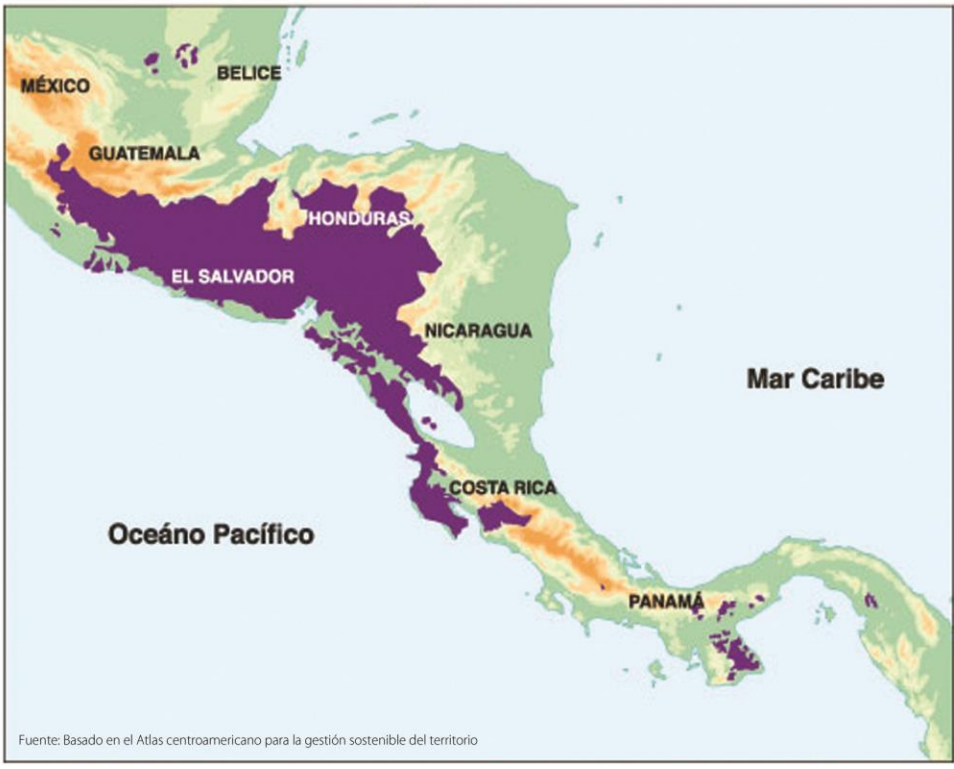
\includegraphics[width=0.5\textwidth]{Docs/Mapa_CS}
    \caption{\small \textit{Dry Corridor Central America}, Situation Report, June 2016, \textbf{FAO}}
    \label{fig:my_label}
\end{figure}

\end{frame}

\begin{frame}{Días sin lluvia}
\begin{figure}
    \centering
    \includegraphics{}
    \caption{Caption}
    \label{fig:my_label}
\end{figure}    
\end{frame}

\end{document}
